\documentclass{ctexart}
\usepackage{amsmath}
\usepackage{float}
\usepackage{xcolor}
\usepackage{tikz}
\usepackage{tikz-3dplot}
\usetikzlibrary{decorations.pathreplacing}%使用大括号
\usetikzlibrary{calligraphy} %calligraphy 书法风格
% \usetikzlibrary{positioning}
\usetikzlibrary{calc}
\usetikzlibrary{backgrounds} %特定的绘图操作置于背景层
\usetikzlibrary{3d}


\usepackage{fancyhdr}
\pagestyle{fancy}
\fancyhf{} % 清空页眉页脚的默认设置
\renewcommand{\headrulewidth}{0pt} % 去除页眉横线
\renewcommand{\footrulewidth}{0pt} % 去除页脚横线
% 在页脚中央添加版权信息
\fancyfoot[C]{\copyright\ 2025 钱皓楠\ -\ 保留所有权利}

% 去除页眉和页脚的横线

\begin{document}


\section{棱柱}
棱柱的底面边数是 $n$, 则这个棱柱有 $3n$ 条棱, $2+n$ 个面.

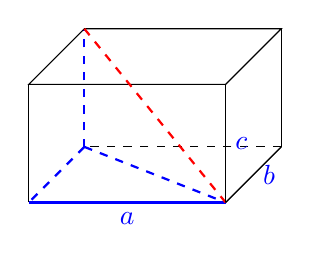
\begin{tikzpicture}[scale=0.5,
    y={(-0.353cm,-0.353cm)}, % 设置 x 轴方向
    x={(1cm,0cm)},            % 设置 y 轴方向
    z={(0cm,1cm)}             % 设置 z 轴方向
]%斜二测画法
    % 定义矩体的尺寸
    \def\a{5} % 长
    \def\b{4} % 宽
    \def\c{3} % 高

    % 定义顶点
    \coordinate (D) at (0,0,0);
    \coordinate (C) at (\a,0,0);
    \coordinate (B) at (\a,\b,0);
    \coordinate (A) at (0,\b,0);
    \coordinate (D') at (0,0,\c);
    \coordinate (C') at (\a,0,\c);
    \coordinate (B') at (\a,\b,\c);
    \coordinate (A') at (0,\b,\c);

    % 绘制底面
    \draw [blue,thick] (A) -- (B) ;
    \draw (B) -- (C) ;
    \draw[dashed] (C) -- (D) ;
    \draw[dashed,blue,thick] (D) -- (A) ;
    % 绘制侧面
    \draw[dashed,blue,thick] (D) -- (D');
    \draw (C) -- (C');
    \draw (B) -- (B');
    \draw (A) -- (A');
    % 绘制顶面
    \draw (D') -- (C') -- (B') -- (A') -- cycle;

    \draw[dashed,blue,thick] (D) -- (B);%底面对角线
    \draw[dashed,red,thick] (D') -- (B);%体对角线

    % % 标注顶点名称
    % \node[below left] at (A) {$A$};
    % \node[below right] at (B) {$B$};
    % \node[below right] at (C) {$C$};
    % \node[above left] at (D) {$D$};

    % \node[below left] at (A') {$A'$};
    % \node[below right] at (B') {$B'$};
    % \node[above right] at (C') {$C'$};
    % \node[above left] at (D') {$D'$};
% \draw (A) -- (B) node[midway, below,blue] {$a$};
    % 在 A 和 B 中间下方标注字母 a
\node[below, blue] at ($(A)!0.5!(B)$) {$a$};
% \node[left=0.3pt,red] at ($(D)!0.5!(B)$) {\tiny $\sqrt{a^2+b^2}$};
\draw (B) -- (C) node[midway, right,blue] {$b$};
\draw (B) -- (B') node[midway, right,blue] {$c$};
\end{tikzpicture}




长宽高分别为$a,b,c$的长方体\textcolor{red}{对角线}的长度为 
\[
\sqrt{a^2+b^2+c^2}.
\]


\section{棱锥}
% \subsection{定义}
\subsection{棱锥的定义}:

\begin{center}
  % \usetikzlibrary{decorations.pathreplacing}%使用大括号
% \usetikzlibrary{calligraphy} %calligraphy 书法风格
% % \usetikzlibrary{positioning}
% \usetikzlibrary{calc}
% \usetikzlibrary{backgrounds} %特定的绘图操作置于背景层
% \usetikzlibrary{3d}

% 将代码中的顶点名称 A、B、C、D 替换为 D、C、B、A
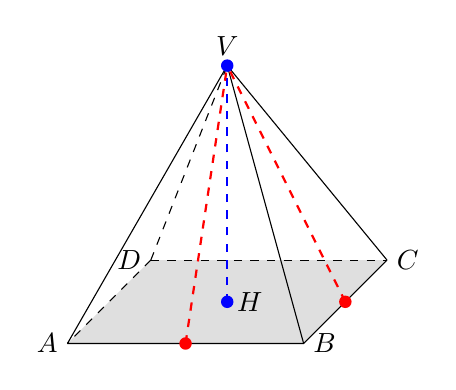
\begin{tikzpicture}[scale=3,
    y={(-0.353cm,-0.353cm)}, % 设置 x 轴方向
    x={(1cm,0cm)},            % 设置 y 轴方向
    z={(0cm,1cm)}             % 设置 z 轴方向
]%斜二测画法
\coordinate (D) at (0,0,0);
\coordinate (C) at (1,0,0);
\coordinate (B) at (1,1,0);
\coordinate (A) at (0,1,0);
\coordinate (V) at (0.5,0.5,1);

\coordinate (H) at (0.5,0.5,0);
% 计算中点
\coordinate (H') at ($(A)!0.5!(B)$);
\coordinate (H'') at ($(C)!0.5!(B)$);
%填充底面
\fill[lightgray,opacity=0.5] (D) -- (C) -- (B) -- (A) -- cycle;

% 绘制底面
\draw (C) -- (B) -- (A);

% 绘制侧面
\draw[dashed] (D) -- (V);
\draw[dashed] (D) -- (A);
\draw[dashed] (D) -- (C);
\draw (C) -- (V);
\draw (B) -- (V);
\draw (A) -- (V);


\draw[thick,blue,dashed] (H) -- (V); %棱柱的高

\draw[thick,red,dashed] (H') -- (V); %棱柱的斜高
\draw[thick,red,dashed] (H'') -- (V); %棱柱的斜高

% 标记顶点
\node[ left] at (D) {$D$};
\node[ right] at (C) {$C$};
\node[ right] at (B) {$B$};
\node[left] at (A) {$A$};
\node[above] at (V) {$V$};
\node[right] at (H) {$H$};

%绘制圆点
\fill[blue] (V) circle (0.75pt);
\fill[blue] (H) circle (0.75pt);
\fill[red] (H') circle (0.75pt);
\fill[red] (H'') circle (0.75pt);
% \node[circle, fill=blue, inner sep=1.5pt] at (V) {};
% \node[circle, fill=blue, inner sep=1.5pt] at (H) {};
\end{tikzpicture}
  
\end{center}


这是一个正四棱锥,蓝色的线段是\textcolor{blue}{高},记为\textcolor{blue}{$h$},而红色的线段是\textcolor{red}{斜高},记为\textcolor{red}{$h'$}.


棱锥的体积公式: 
\[
V =\frac{1}{3} S_\text{底} h.
\]

正棱锥的侧面积公式: 
\[
S_\text{正棱锥侧} =\frac{1}{2} c h'.
\]
故正棱锥表面积公式为
\[
    S_\text{正棱锥表}  =S_\text{正棱锥侧}+S_\text{底} = \frac{1}{2} c h'+S_\text{底}.
\]



\subsection{常见的棱锥}

\begin{figure}[H]
\centering
% 将代码中的顶点名称 A、B、C、D 替换为 D、C、B、A
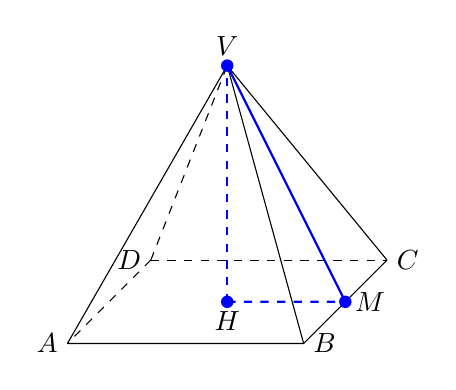
\begin{tikzpicture}[scale=3,
    y={(-0.353cm,-0.353cm)}, % 设置 x 轴方向
    x={(1cm,0cm)},            % 设置 y 轴方向
    z={(0cm,1cm)}             % 设置 z 轴方向
]%斜二测画法
\coordinate (D) at (0,0,0);
\coordinate (C) at (1,0,0);
\coordinate (B) at (1,1,0);
\coordinate (A) at (0,1,0);
\coordinate (V) at (0.5,0.5,1);

\coordinate (H) at (0.5,0.5,0);
% 计算中点
\coordinate (H') at ($(A)!0.5!(B)$);
\coordinate (H'') at ($(C)!0.5!(B)$);
\coordinate (M) at ($(C)!0.5!(B)$);
% %填充底面
% \fill[lightgray,opacity=0.5] (D) -- (C) -- (B) -- (A) -- cycle;

% 绘制底面
\draw (C) -- (B) -- (A);

% 绘制侧面
\draw[dashed] (D) -- (V);
\draw[dashed] (D) -- (A);
\draw[dashed] (D) -- (C);
\draw (C) -- (V);
\draw (B) -- (V);
\draw (A) -- (V);


\draw[thick,blue,dashed] (H) -- (V); %棱柱的高
\draw[thick,blue,dashed] (H) -- (M); %
\draw[thick,blue] (V) -- (M); %斜高

% \draw[thick,red,dashed] (H') -- (V); %棱柱的斜高
% \draw[thick,red,dashed] (H'') -- (V); %棱柱的斜高

% 标记顶点
\node[ left] at (D) {$D$};
\node[ right] at (C) {$C$};
\node[ right] at (B) {$B$};
\node[left] at (A) {$A$};
\node[above] at (V) {$V$};
\node[below] at (H) {$H$};
\node[right] at (M) {$M$};


%绘制圆点
\fill[blue] (V) circle (0.75pt);
\fill[blue] (H) circle (0.75pt);
\fill[blue] (M) circle (0.75pt);
% \fill[red] (H') circle (0.75pt);
% \fill[red] (H'') circle (0.75pt);
\end{tikzpicture}
\caption{正四棱锥}
\end{figure}
线段 $VH$ 是正四棱锥的高, $M$ 是 $BC$ 边上的中点,则有,
$$ |HM|^2 + |VH|^2 = |VM|^2. $$

\begin{figure}[H]
    \centering
    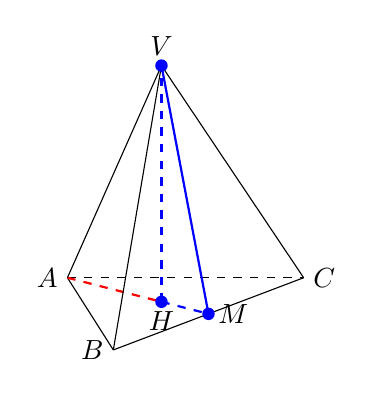
\begin{tikzpicture}[scale=3,
        y={(-0.353cm,-0.353cm)}, % 设置 x 轴方向
        x={(1cm,0cm)},            % 设置 y 轴方向
        z={(0cm,1cm)}             % 设置 z 轴方向
    ]%斜二测画法
    % 定义底面正三角形的顶点
    \coordinate (A) at (0,0,0);
    \coordinate (C) at (1,0,0);
    \coordinate (B) at (0.5,{sqrt(3)/2},0);
    
    % 定义顶点 V
    \coordinate (V) at (0.5,{sqrt(3)/6},1);
    
    % 计算底面中心 H
    \coordinate (H) at (0.5,{sqrt(3)/6},0);
    
    % 计算各边中点
    \coordinate (H') at ($(A)!0.5!(C)$);
    \coordinate (M) at ($(C)!0.5!(B)$);
    \coordinate (H''') at ($(B)!0.5!(A)$);
    
    % 绘制底面
    \draw[dashed] (A) -- (C);
    \draw (A) -- (B);
    \draw (C) -- (B);

    %%高
    \draw[dashed,red,thick] (A) -- (H);
    \draw[dashed,blue,thick] (H) -- (M);


    
    % 绘制侧面
    \draw (A) -- (V);
    \draw (C) -- (V);
    \draw (B) -- (V);
    %% 斜高
    \draw[blue,thick] (V) -- (M);
    % 棱锥的高
    \draw[thick,blue,dashed] (H) -- (V); 
    
    % 标记顶点
    \node[left] at (A) {$A$};
    \node[right] at (C) {$C$};
    \node[left] at (B) {$B$};
    \node[above] at (V) {$V$};
    \node[below] at (H) {$H$};

    \node[right] at (M) {$M$};

    
    % 绘制圆点
    \fill[blue] (V) circle (0.75pt);
    \fill[blue] (H) circle (0.75pt);
    \fill[blue] (M) circle (0.75pt);
    \end{tikzpicture}
    \caption{正三棱锥}
\end{figure} 
 

线段 $VH$ 是正三棱锥的高, $M$ 是 $BC$ 边上的中点,$H$ 是底面正三角形 $\triangle ABC$ 的中心. 则 $\frac{|AH|}{|HM|} = 2$,即 $|HM|  = \frac{1}{3} |AM|$.同样的有,
$$ |HM|^2 + |VH|^2 = |VM|^2. $$
    
\begin{figure}[H]
    \centering
    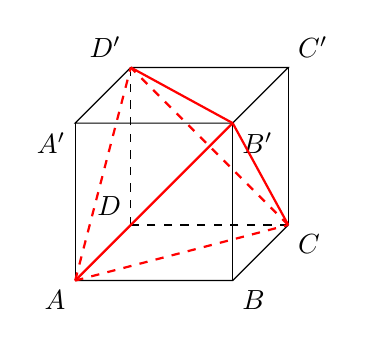
\begin{tikzpicture}[scale=0.5,
        y={(-0.353cm,-0.353cm)}, % 设置 x 轴方向
        x={(1cm,0cm)},            % 设置 y 轴方向
        z={(0cm,1cm)}             % 设置 z 轴方向
    ]%斜二测画法
        % 定义矩体的尺寸
        \def\a{4} % 长
        \def\b{4} % 宽
        \def\c{4} % 高

        % 定义顶点
        \coordinate (D) at (0,0,0);
        \coordinate (C) at (\a,0,0);
        \coordinate (B) at (\a,\b,0);
        \coordinate (A) at (0,\b,0);
        \coordinate (D') at (0,0,\c);
        \coordinate (C') at (\a,0,\c);
        \coordinate (B') at (\a,\b,\c);
        \coordinate (A') at (0,\b,\c);

        % 绘制底面
        \draw (C) -- (B) -- (A) ;
        \draw[dashed] (C) -- (D) ;
        \draw[dashed] (D) -- (A) ;
        % 绘制侧面
        \draw[dashed] (D) -- (D');
        \draw (C) -- (C');
        \draw (B) -- (B');
        \draw (A) -- (A');
        % 绘制顶面
        \draw (D') -- (C') -- (B') -- (A') -- cycle;

        % 标注顶点名称
        \node[below left] at (A) {$A$};
        \node[below right] at (B) {$B$};
        \node[below right] at (C) {$C$};
        \node[above left] at (D) {$D$};

        \node[below left] at (A') {$A'$};
        \node[below right] at (B') {$B'$};
        \node[above right] at (C') {$C'$};
        \node[above left] at (D') {$D'$};
        % 绘制正四面体
        \draw[red,thick] (D') -- (B');
        \draw[red,thick] (A) -- (B');
        \draw[red,thick] (C) -- (B');
        \draw[dashed,red,thick] (A) -- (C);
        \draw[dashed,red,thick] (A) -- (D');
        \draw[dashed,red,thick] (C) -- (D');
        % \draw[dashed,red,thick] (D') -- (B);
    \end{tikzpicture}
    \caption{正六面体中的正四面体}
\end{figure}

\section{圆柱}

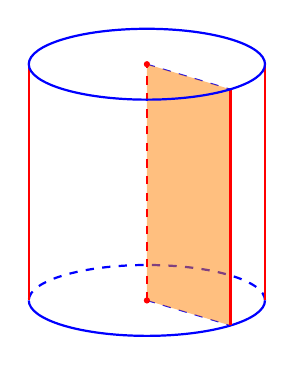
\begin{tikzpicture}[scale=1.5,
    y={(0cm,-0.3cm)}, % 设置 x 轴方向
    x={(1cm,0cm)},            % 设置 y 轴方向
    z={(0cm,1cm)}             % 设置 z 轴方向
]%斜二测画法
    % 定义圆柱的参数
    \def\radius{1} % 圆柱底面半径
    \def\height{2} % 圆柱的高度
    \coordinate (O') at (0,0,\height);
    \coordinate (O) at (0,0,0);

    %上圆上一点
    \coordinate (A') at ({\radius*sqrt(2)/2},{\radius*sqrt(2)/2},\height);

    %下圆上一点
    \coordinate (A) at ({\radius*sqrt(2)/2},{\radius*sqrt(2)/2},0);


    \fill[orange,opacity=0.5](A') -- (A) -- (O) -- (O') -- cycle; %填充颜色

        % 绘制母线
        \begin{scope}
            \draw[thick,red] (\radius,0,0) -- (\radius,0,\height);
            \draw[thick,red] (-\radius,0,0) -- (-\radius,0,\height);
        \end{scope}
        % 绘制高线
        \begin{scope}
            \fill[red] (0,0,0) circle (0.75pt);  % 绘制一个点测试一下 
            \fill[red] (0,0,\height) circle (0.75pt);  % 绘制一个点测试一下 
            \draw[thick,red,dashed] (0,0,0) -- (0,0,\height);
            \draw[thick,red] (A) -- (A');
            \end{scope}

        % 绘制顶面圆
        \begin{scope}
            %绘制一个圆
            % \draw(0,0,\height) circle (\radius);
            %上半圆
            \draw [blue,thick] (\radius,0,\height) arc (0:-180:\radius) ;
            \draw [blue,thick] (\radius,0,\height) arc (0:180:\radius) ;
        \end{scope}

      
        % 绘制底面圆
        \begin{scope}[on background layer]
            \draw [blue,thick,dashed] (\radius,0,0) arc (0:-180:\radius) ;
            \draw [blue,thick] (\radius,0,0) arc (0:180:\radius) ;
        \end{scope}

        % 绘制底面顶面半径
        \begin{scope}[on background layer]
            %绘制一个圆
            % \draw(0,0,\height) circle (\radius);
            \draw [blue,thin,dashed] (O) -- (A) ;
            \draw [blue,thin,dashed] (O') -- (A') ;
            % \draw [blue,thick] (\radius,0,\height) arc (0:180:\radius) ;
        \end{scope}

    



        % % 绘制括号
        % \begin{scope}[on background layer]
        %     \draw[decorate,decoration={brace,amplitude=10pt},thick] (0-0.1,0,0) -- (0-0.1,0,\height);
        % \end{scope}



\end{tikzpicture}



圆柱轴截面\\
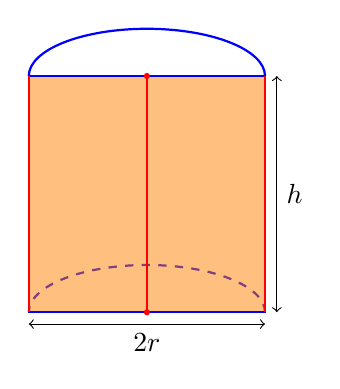
\begin{tikzpicture}[scale=1.5,
    y={(0cm,-0.4cm)}, % 设置 x 轴方向
    x={(1cm,0cm)},            % 设置 y 轴方向
    z={(0cm,1cm)}             % 设置 z 轴方向
]%斜二测画法
    % 定义圆柱的参数
    \def\radius{1} % 圆柱底面半径
    \def\height{2} % 圆柱的高度
    \coordinate (O') at (0,0,\height);
    \coordinate (O) at (0,0,0);
    \coordinate (R') at (\radius,0,\height);
    \coordinate (R) at (\radius,0,0);
    \coordinate (R'') at (-\radius,0,\height);
    \coordinate (R''') at (-\radius,0,0);


    % %上圆上一点
    % \coordinate (A') at ({\radius*sqrt(2)/2},{\radius*sqrt(2)/2},\height);

    % %下圆上一点
    % \coordinate (A) at ({\radius*sqrt(2)/2},{\radius*sqrt(2)/2},0);


    % \fill[orange,opacity=0.5](A') -- (A) -- (O) -- (O') -- cycle; %填充颜色

    % \fill[orange,opacity=0.5](O') -- (O) -- (R) -- (R') -- cycle; %填充颜色
    \fill[orange,opacity=0.5](R) -- (R') -- (R'') -- (R''') -- cycle; %填充颜色
    \draw[blue,thick] (R) -- (R') -- (R'') -- (R''') -- cycle; %填充颜色



    \draw[<->] ($(R''')+(0,0,-0.1)$)-- ($(R)+(0,0,-0.1)$) node[midway,below]{\( 2r \)};

    \draw[<->] ($(R)+(0.1,0,0)$)-- ($(R')+(0.1,0,0)$) node[midway,right]{\( h \)};
    % ($(0,0) + (1,1)$)

        % 绘制母线
        \begin{scope}
            \draw[thick,red] (\radius,0,0) -- (\radius,0,\height);
            \draw[thick,red] (-\radius,0,0) -- (-\radius,0,\height);
        \end{scope}
        % 绘制高线
        \begin{scope}
            \fill[red] (0,0,0) circle (0.75pt);  % 绘制一个点测试一下 
            \fill[red] (0,0,\height) circle (0.75pt);  % 绘制一个点测试一下 
            \draw[thick,red] (0,0,0) -- (0,0,\height);
            \end{scope}

        % 绘制顶面圆
        \begin{scope}
            %绘制一个圆
            % \draw(0,0,\height) circle (\radius);
            %上半圆
            \draw [blue,thick] (\radius,0,\height) arc (0:-180:\radius) ;
            % \draw [blue,thick] (\radius,0,\height) arc (0:180:\radius) ;
        \end{scope}

      
        % 绘制底面圆
        \begin{scope}[on background layer]
            \draw [blue,thick,dashed] (\radius,0,0) arc (0:-180:\radius) ;
            % \draw [blue,thick] (\radius,0,0) arc (0:180:\radius) ;
        \end{scope}

\end{tikzpicture}






\section{圆锥}
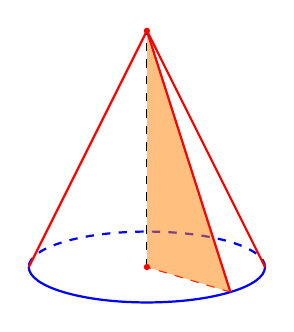
\begin{tikzpicture}[scale=1.5,
    y={(0cm,-0.3cm)}, % 设置 x 轴方向
    x={(1cm,0cm)},            % 设置 y 轴方向
    z={(0cm,1cm)}             % 设置 z 轴方向
]
    % 定义圆柱的参数
    \def\radius{1} % 圆锥底面半径
    \def\height{2} % 圆锥的高度
    % 一些坐标
    \coordinate (O') at (0,0,\height);
    \coordinate (O) at (0,0,0);
    %上圆上一点
    \coordinate (A') at ({\radius*sqrt(2)/2},{\radius*sqrt(2)/2},\height);
    %下圆上一点
    \coordinate (A) at ({\radius*sqrt(2)/2},{\radius*sqrt(2)/2},0);
        % 底面半径
        \draw[thin,dashed,red] (A) -- (O);
        % 绘制底面圆
        \begin{scope}
            \draw [blue,thick,dashed] (\radius,0,0) arc (0:-180:\radius) ;
            \draw [blue,thick] (\radius,0,0) arc (0:180:\radius) ;

        \end{scope}
        \fill[orange,opacity=0.5] (A) -- (O) -- (O') -- cycle; %填充颜色
        % 绘制母线
        \begin{scope}
            \draw[thick,red] (\radius,0,0) -- (O');
            \draw[thick,red] (-\radius,0,0) -- (O');
            \draw[thick,red] (A) -- (O');
        \end{scope}
        

        % 绘制高线
        \begin{scope}
            \draw[thin,dashed] (0,0,0) -- (0,0,\height);
            \fill[red] (0,0,0) circle (0.75pt);  % 绘制一个点测试一下 
            \fill[red] (0,0,\height) circle (0.75pt);  % 绘制一个点测试一下 
        \end{scope}
\end{tikzpicture}


设圆锥的底面半径为 $r$ ,母线长为 $l$ , 则其底面积为  $\pi r^2$.侧面展开的扇形的圆弧长为 $2 \pi r$ ,则侧面积为 $\frac{1}{2}(2 \pi r) l = \pi r l$.







\subsection{圆锥展开图}

%圆锥展开图
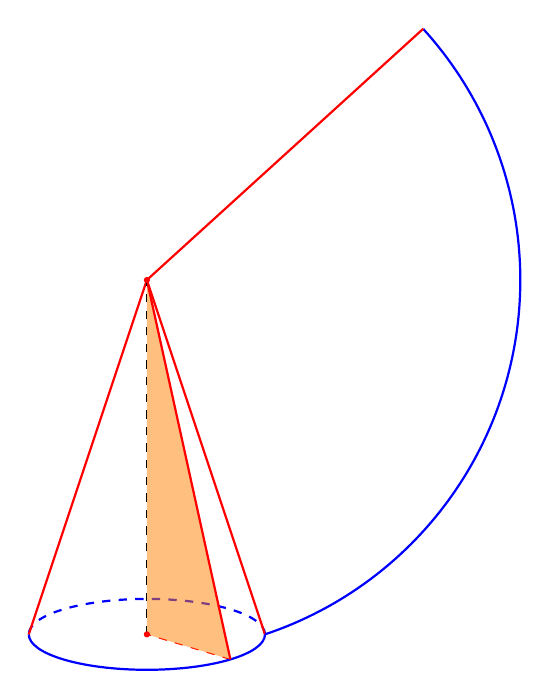
\begin{tikzpicture}[scale=1.5,
    y={(0cm,-0.3cm)}, % 设置 x 轴方向
    x={(1cm,0cm)},            % 设置 y 轴方向
    z={(0cm,1cm)}             % 设置 z 轴方向
]
    % 定义圆柱的参数
    \def\radius{1} % 圆锥底面半径
    \def\height{3} % 圆锥的高度
    \pgfmathsetmacro{\expandradius}{sqrt(\radius*\radius + \height *\height)} %展开图弧长

    \pgfmathsetmacro{\expandarc}{2*pi*\radius/\expandradius} %展开图圆心角

    \pgfmathsetmacro{\resultAtan}{atan(\radius / \height )}
    % 将弧度转换为角度

    % 一些坐标
    \coordinate (O') at (0,0,\height);
    \coordinate (O) at (0,0,0);
    %上圆上一点
    \coordinate (A') at ({\radius*sqrt(2)/2},{\radius*sqrt(2)/2},\height);
    %下圆上一点
    \coordinate (A) at ({\radius*sqrt(2)/2},{\radius*sqrt(2)/2},0);
        % 底面半径
        \draw[thin,dashed,red] (A) -- (O);
        % 绘制底面圆
        \begin{scope}
            \draw [blue,thick,dashed] (\radius,0,0) arc (0:-180:\radius) ;
            \draw [blue,thick] (\radius,0,0) arc (0:180:\radius) ;

        \end{scope}
        \fill[orange,opacity=0.5] (A) -- (O) -- (O') -- cycle;
        % 绘制母线
        \begin{scope}
            \draw[thick,red] (\radius,0,0) -- (O');
            \draw[thick,red] (-\radius,0,0) -- (O');
            \draw[thick,red] (A) -- (O');
        \end{scope}
        

        % 绘制高线
        \begin{scope}
            \draw[thin,dashed] (0,0,0) -- (0,0,\height);
            \fill[red] (0,0,0) circle (0.75pt);  % 绘制一个点测试一下 
            \fill[red] (0,0,\height) circle (0.75pt);  % 绘制一个点测试一下 
        \end{scope}


    % 绘制展开图圆弧
    \begin{scope}[canvas is xz plane at y=0]
        % \draw [blue,thick] (\radius,0,0) arc [start angle=-\expandarc/2 r, end angle=\expandarc/2 r, radius=\expandradius];
        \draw[blue, thick] plot[domain=0 r:\expandarc r,samples=100] ({\expandradius*cos(\x - pi/2 r +\resultAtan )},{\expandradius*sin(\x - pi/2 r +\resultAtan  )+\height});
    \end{scope}

    % - pi r +\atan(\radius/\height) r

    % 绘制展开图扇形的边
    \begin{scope}
        % \draw[thick,red] (\radius,0,2 *\height) -- (O');
        \draw[thick,red] ({\expandradius*cos(\expandarc r - pi/2 r +\resultAtan )},0,{\expandradius*sin(\expandarc r - pi/2 r +\resultAtan  )+\height}) -- (O');
        % \draw[thick,red] (-\radius,0,0) -- (O');
        % \draw[thick,red] (A) -- (O');
    \end{scope}

    % \node[red, align=center] at (4,0) {\expandradius};
    % \node[red, align=center] at (4,1) { \pgfmathatan{1} \pgfmathresult};
\end{tikzpicture}
% 圆弧的圆心角为 $\farc{2 \pi r }{l}$
\section{球}



\begin{figure}[H]
    \centering
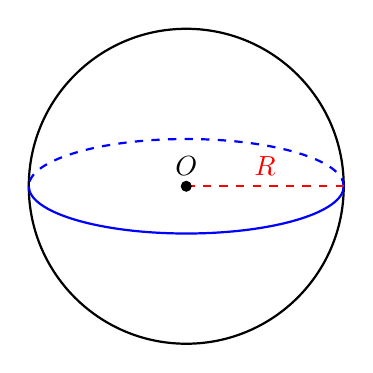
\begin{tikzpicture}[thick]
    % \shade[ball color = gray!40, opacity = 0.4] (0,0) circle (2cm);
    \draw (0,0) circle (2cm);
    \draw[blue] (-2,0) arc (180:360:2 and 0.6);
    \draw[dashed,blue] (2,0) arc (0:180:2 and 0.6);
    \draw[dashed,red] (0,0 ) -- node[above]{$R$} (2,0);
    \fill[fill=black] (0,0) circle (2pt);
    \node[above] at (0,0) {$O$};
\end{tikzpicture}

\caption{球的大圆}
\end{figure} 
如上图所示,经过球心的球截面称之为大圆,其半径$R$和球的半径相同.



\begin{figure}[H]
    \centering
  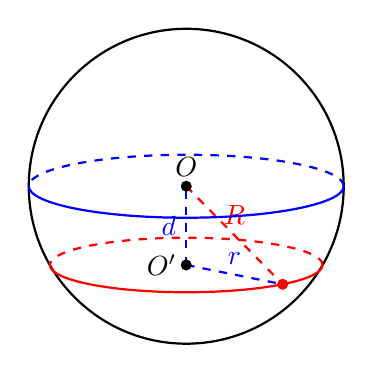
\begin{tikzpicture}[scale=2,
    y={(-0,-0.2cm)}, % 设置 x 轴方向
    x={(1cm,0cm)},            % 设置 y 轴方向
    z={(0cm,1cm)}             % 设置 z 轴方向
]%斜二测画法
    % 定义圆柱的参数
    \def\radius{1} % 圆锥底面半径
    \def\height{2} % 圆锥的高度
    %这只是个一个文本替换
    % \def\littleradius{{\radius*sqrt(3)/2}} % 底面小圆半径
    \pgfmathsetmacro{\littleradius}{\radius*sqrt(3)/2}


    %球心
    \coordinate (O) at (0,0,0);
    %小圆圆心
    \coordinate (O') at (0,0,-\radius/2);
    %小圆上一点
    \coordinate (A) at ({\littleradius*sqrt(2)/2},{\littleradius*sqrt(2)/2},-\radius/2);


    \node[above] at (O) {$O$};
    \node[left] at (O') {$O'$};
    % \node[below] at (A) {$A$};
    \draw[dashed,red,thick] (O) -- node[above]{$R$} (A);
    \draw[dashed,blue,thick] (O') -- node[above]{$r$} (A);
    \draw[dashed,blue,thick] (O') -- node[left]{$d$} (O);



      
        % 绘制正面圆
        \begin{scope}[canvas is xz plane at y=0]
            \draw[thick] (0,0) circle (\radius);
        \end{scope}


        % 绘制水平圆
        \begin{scope}[canvas is xy plane at z=0]
            \draw [blue,thick,dashed] (\radius,0) arc (0:-180:\radius) ;
            \draw [blue,thick] (\radius,0) arc (0:180:\radius) ;
        \end{scope}


        % 绘制水平小圆 这个小圆刚好是圆心下降一半的半径的位置
        \begin{scope}[canvas is xy plane at z=-\radius/2]
            \draw [red,thick,dashed] (\littleradius,0) arc (0:-180:\littleradius) ;
            \draw [red,thick] (\littleradius,0) arc (0:180:\littleradius) ;
        \end{scope}


        % 绘制圆心
        \begin{scope}
            \fill[fill=black] (O) circle (1pt);
            \fill[fill=black] (O') circle (1pt);
            \fill[fill=red] (A) circle (1pt);
        \end{scope}
        

        
        %问题 怎么根据比例绘制圆弧上的点,我想要在圆弧上描点来连接球心.


        % 绘制竖直圆 % 竖直圆有问题,不绘制
        % 因为书本上的球,并不是使用斜二测画法绘制的
        % \begin{scope}[canvas is yz plane at x=0]
        %     \draw [blue,thick,dashed] (\radius,0,0) arc (0:-180:\radius) ;
            
        %     \draw [blue,thick] (\radius,0,0) arc (0:180:\radius) ;
        % \end{scope}
\end{tikzpicture}
\caption{球的小圆}
\end{figure} 

如图,球的半径为 $R$ , 小圆的半径为 $r$ ,球心 $O$ 到小圆圆面的距离为 $d$,则根据勾股定理有
$$
r^2 + d^2 =R^2.
$$
\clearpage


\section{补充知识}
\subsection{等边三角形相关结论}
\begin{center}
    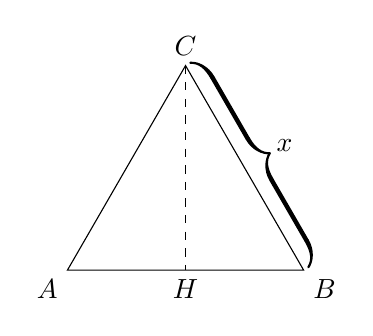
\begin{tikzpicture}
        % 定义正三角形的边长
        \def\sideLength{3}

        % 定义点
        \coordinate (A) at (0,0);
        \coordinate (B) at (\sideLength,0);
        \coordinate (C) at (\sideLength/2,{sqrt(3)*\sideLength/2});
        % 计算 AB 的中点
        \coordinate (H) at ($(A)!0.5!(B)$);

        % 绘制正三角形
        \draw (A) -- (B) -- (C) -- cycle;
        \draw[dashed] (C) -- (H);

        % 标记顶点
        \node[below left] at (A) {$A$};
        \node[below right] at (B) {$B$};
        \node[above] at (C) {$C$};
        \node[below] at (H) {$H$};
        \draw[decorate,decoration={calligraphic brace,amplitude=3mm,raise=2pt},ultra thick] (C) -- (B); 
        %raise 表示让括号位移一点 amplitude 控制花括号的弯度程度 
        % calligraphic brace 有粗细变换的括号
        \node at ($(C)!0.5!(B)$) [above=8pt,right=8pt] {$x$};
    \end{tikzpicture}
\end{center}

一个正三角形的边长为$x$,则其高为$\frac{\sqrt{3}}{2} x$, 则其面积为 $\frac{\sqrt{3}}{4} x^2$.

\begin{center}
    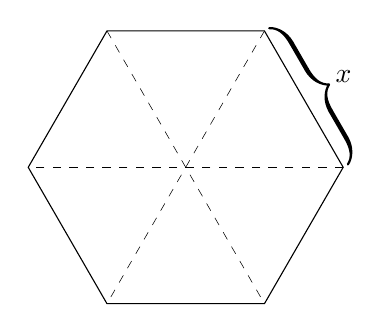
\begin{tikzpicture}[scale=2]
        % 定义正六边形外接圆半径
        \def\radius{1}
        % 定义正六边形顶点坐标
        \coordinate (A) at (\radius, 0);
        \coordinate (B) at ({0.5 * \radius}, {sqrt(3) * 0.5 * \radius});
        \coordinate (C) at ({-0.5 * \radius}, {sqrt(3) * 0.5 * \radius});
        \coordinate (D) at (-\radius, 0);
        \coordinate (E) at ({-0.5 * \radius}, {-sqrt(3) * 0.5 * \radius});
        \coordinate (F) at ({0.5 * \radius}, {-sqrt(3) * 0.5 * \radius});

        % % 绘制顶点
        % \foreach \point in {A, B, C, D, E, F} {
        %     \fill (\point) circle (2pt);
        % }

        % 绘制正六边形的边
        \draw (A) -- (B) -- (C) -- (D) -- (E) -- (F) -- cycle;
        \draw[dashed,line width=0.2pt] (A)  -- (D) ;
        \draw[dashed,line width=0.2pt] (B)  -- (E) ;
        \draw[dashed,line width=0.2pt] (C)  -- (F) ;

        % % 标记顶点
        % \foreach \point in {A, B, C, D, E, F} {
        %     \node[above right] at (\point) {$\point$};
        % }

        \draw[decorate,decoration={calligraphic brace,amplitude=3mm,raise=2pt},ultra thick] (B) -- (A); 
        \node at ($(A)!0.5!(B)$) [above=8pt,right=8pt] {$x$};
    \end{tikzpicture}
\end{center}


因为一个正六边形能分割成$6$个全等的正三角形,所以边长为$x$的正六边形的面积是 $6 \times \frac{\sqrt{3}}{4} x^2  $.






\begin{figure}[H]
    \centering
	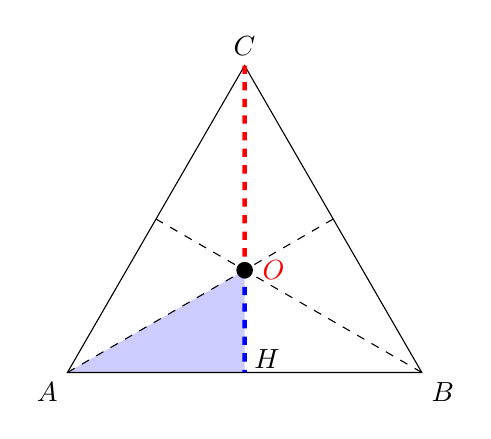
\begin{tikzpicture}[scale=1.5]
    % 定义正三角形的边长
    \def\sideLength{3}
    % 定义点
    \coordinate (A) at (0,0);
    \coordinate (B) at (\sideLength,0);
    \coordinate (C) at (\sideLength/2,{sqrt(3)*\sideLength/2});
    % 计算 AB 的中点
    \coordinate (H) at ($(A)!0.5!(B)$);
    \coordinate (O) at ($(H)!0.3333!(C)$); % 中点

    %填涂区域
    \fill[blue!20] (A) -- (O) -- (H) -- cycle;




    % 绘制正三角形
    \draw (A) -- (B) -- (C) -- cycle;
    % \draw[dashed] (C) -- (H);
    \draw[dashed,ultra thick, red] (C) -- (O);
    \draw[dashed,ultra thick,blue] (O) -- (H);
    % \draw[dashed,thick,blue] (C) -- (O);
    \draw[dashed] (A) -- ($(C)!0.5!(B)$);
    \draw[dashed] (B) -- ($(C)!0.5!(A)$);


    % 标记顶点
    \node[below left] at (A) {$A$};
    \node[below right] at (B) {$B$};
    \node[above] at (C) {$C$};
    \node[above=5pt,right] at (H) {$H$};
    \node[right=3pt,red] at (O) {$O$};

    \fill (O) circle (2pt);%填涂测试
\end{tikzpicture}

\end{figure}
一个正三角形还能被分割成如图所示的$6$个全等的直角三角形,则线段 $|CO|$ 与线段 $|OH|$ 的比值为 $2$\footnote{你能证明吗?}.

\subsection{弧度制的复习}



\end{document}